\documentclass[a4paper,12pt]{article} %Indica a classe do documento
\usepackage[utf8]{inputenc} % Codificação do arquivo
\usepackage[english,brazil]{babel} % Idiomas do documento
\usepackage{hyperref} % Links clicáveis, todos em azul
\hypersetup{
        colorlinks=true,
        linkcolor=blue,
        urlcolor=blue,
        citecolor=blue
}
\usepackage{pdfpages} % Pacote para o anexo dos pdfs ao final do documento
\usepackage{graphicx} % Incluir imagens
\usepackage{fancyhdr} % Estilo de cabeçalho e rodapé
\usepackage{setspace} % Espaçamento entre linhas mais inteligente
%\usepackage{indentfirst} % Indenta o primeiro parágrafo de cada seção. Descomente para utilizá-lo
\usepackage{xspace} % Espaçamento inteligente
\usepackage[style=nature, intitle=true,articletitle=true,doi=false, url=false, isbn=false, maxnames=20]{biblatex} % Estilo de citação bibliográfica baseado na revista Nature
\usepackage{geometry} % Configuração das margens
\usepackage{csquotes} % Lida com as aspas do texto e nas citações bibliográficas
\usepackage{lipsum} % Texto fictício para preencher o modelo, comente ou apague essa linha quando não for mais necessário
\usepackage{attachfile} % Anexar arquivos, os comprovantes ao final do documento
\newcommand{\listadecomprovantes}{} % Lista para armazenar os comprovantes
\linespread{1.25} % Espaçamento 1,5 entre linhas
\geometry{a4paper,margin=1.5in} % Configuração das margens do corpo do texto. Com margens largas o texto fica muito bonito e legível, quase como um livro
%% Adicione o arquivo com as referências bibliográficas
\addbibresource{artigos_publicados.bib}
%% Escreva aqui seu nome
\newcommand{\nomeAutor}{Fulane de Tal, PhD}
%% Escreva aqui o nome da cidade
\newcommand{\nomeCidade}{Gotham City}
%% Escreva aqui o seu título
\newcommand{\meuTitulo}{Memorial Circunstanciado}
% contador para os comprovantes
\newcounter{comprovante} 

\newcommand{\comprovante}[1]{%
    \stepcounter{comprovante}%
    \hyperref[comprovante:\thecomprovante]{comprovante \thecomprovante}%
    \xappto{\listadecomprovantes}{%
     \noexpand\clearpage
      \noexpand\subsection*{Comprovante \thecomprovante}%
      \noexpand\addcontentsline{toc}{subsection}{Comprovante \thecomprovante}%
      \noexpand\label{comprovante:\thecomprovante}%
      \noexpand\includegraphics[width=\textwidth,height=\textheight,keepaspectratio]{#1}%
    }%
}

\begin{document}
\emergencystretch 3em
\newgeometry{top=30mm,bottom=20mm,left=30mm,right=20mm} %margens curtas para a capa
\begin{titlepage}
\setlength{\headheight}{80pt}
    \thispagestyle{fancy} % Aplica o estilo fancy apenas a esta página
    \fancyhf{}
 \renewcommand{\headrulewidth}{1pt} % Escolhe a espessura da linha horizontal
            \fancyhead[L]{
\includegraphics[height=.9in]{figuras/Gotham_University_Symbol.jpg}}% Insira o arquivo logo da universidade aqui
            \fancyhead[C]{\begin{center} \small \textbf{UNIVERSIDADE ESTADUAL DE GOTHAM CITY\\ INSTITUTO DE CIÊNCIAS BIOLÓGICAS \\ DEPARTAMENTO DE COSMOLOGIA}\end{center}}
            \fancyhead[R]{
\includegraphics[height=1in]{figuras/dc_logo.png}}% Insira o arquivo do timbre aqui

	\vfill
        \begin{center}
        	\vspace*{\fill}      
            % Título do trabalho
            {\linespread{1.5}\Huge \textbf{\meuTitulo} \par}
            
            % Nome do autor

         \vfill
            {\Large \nomeAutor \par}
            
            % Caixa de texto
         \vfill
            \begin{flushright}
                \parbox{0.5\textwidth}{Memorial submetido à apreciação da Banca Examinadora do Concurso Público de Provas e Títulos para provimento efetivo de vaga em cargo integrante da carreira do magistério superior, na Classe A, com a denominação de Professor Adjunto A, Nível 1, área de conhecimento \textbf{Biologia de Kryptonianos} do \textbf{Departamento de Cosmologia} do Instituto de Ciências Biológicas da Universidade Estadual de Gotham City. \textbf{Edital N\textsuperscript{o} XX/202X}}
            \end{flushright}
            
            
            % Cidade e data
         \vfill

            {\normalsize \nomeCidade, \today \par}
             \vfill

        \end{center}
\end{titlepage}

\restoregeometry

%Escreva seu resumo aqui. Caso não queira um resumo, comente as próximas linhas
\section*{Resumo}
\lipsum[1-2]
\pagestyle{empty}
\newpage

% Adiciona sumário
\renewcommand{\contentsname}{Sumário}
\pagestyle{empty}
\tableofcontents
\clearpage

\pagestyle{fancy}
\fancyhf{}
\fancyhfoffset[R]{0pt} % Adiciona esse comando para ajustar a margem direita
\setlength{\headheight}{16pt}
\renewcommand{\sectionmark}[1]{\markboth{\thesection\,--\,#1}{}}
\fancyhead[L]{\textbf{\leftmark}}
\fancyhead[R]{\thepage}
\setcounter{page}{1}

% As seções estão separadas para melhor organização e são adicionadas de acordo com o comando input

\section{Formação Acadêmica}
\label{sec:formacao}

\lipsum[3-4]

\subsection{Títulos Universitários}
\label{subsec:titulos}  
    \subsubsection{Graduação em Ciências Biológicas pela Universidade Estadual de Pequenópolis (2005--2009)}
   
Em meados de 2005, ingressei no curso de Ciências Biológicas na UEP e me formei em 2009 (\comprovante{comprovantes/graduacao.pdf}). \lipsum[5-6]
    
    \subsubsection{Mestrado em Astrobiologia pela Universidade Federal de Gotham City (2010--2012)}
    
\lipsum[7-8]
    
    \subsubsection{Doutorado em Exobiologia pela Universidade de Metrópolis (2013--2017)}

Meu doutorado, intitulado \foreignquote{english}{Systematics and evolution of the Kryptonian species of fish-snakes using high-throughtput sequencing} foi defendido com honras, em 2017.

\lipsum[9-10]
    
\subsection{Estágios de pós-doutoramento}
\label{subsec:posdoc}
    
    \subsubsection{Pós-doutorado pela Universidade Estadual de Metrópolis (2018--atual)}

\lipsum[11-14]


\section{Atividades Científicas}
\label{sec:cientificas}
    \subsection{Publicações}
    \label{subsec:publicacoes}


Meu primeiro artigo científico foi publicado como coautor \cite{jorel2012}, fruto do meu estágio no Departamento de Astrobiologia da UEP sob a orientação do Prof. Dr. Zor-El (\comprovante{comprovantes/artigo.pdf}). \lipsum[15-16]



\section{Atividades Didáticas}
\label{sec:didaticas}

\lipsum[18]

\subsection{Atividades de Ensino}
\label{subsec:ensino}

\lipsum[19-20]


\subsection{Orientações}
\label{subsec:orientacoes}  
 
\lipsum[21-22]

\subsection{Participação em Bancas}

\lipsum[23-24]

\subsection{Cursos e Palestras}
\label{subsec:cursos}  

\lipsum[25-27]


\section{Produção de Conhecimento}
\label{sec:producao}  
\subsection{Bolsas e Projetos de Pesquisa}
\label{subsec:bolsas}  

\lipsum[28-29]

\subsection{Participação em Eventos Científicos}
\label{subsec:eventos}  

\lipsum[30-31]

\subsection{Serviço editorial}
\label{subsec:editorial}  

\lipsum[32-33]



\section{Considerações Finais}
\label{sec:consideracoes}  

\lipsum[34-36]

\begin{figure}[!b]
    \centering
    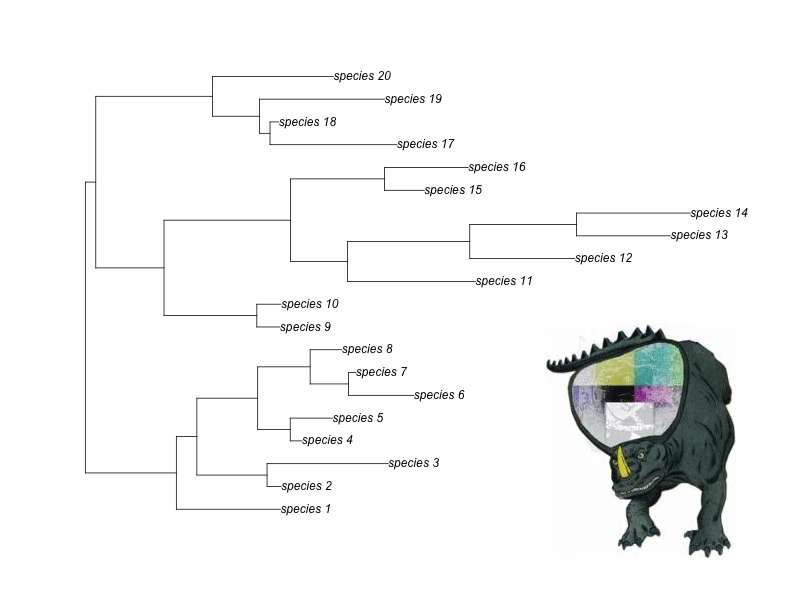
\includegraphics[width=1\textwidth]{figuras/species_krypton.png}
    \caption{\lipsum[37]}
    \label{fig:figura_1}
\end{figure}

\subsection{Perspectivas Futuras}
\label{subsec:perspectivas}  

A figura \ref{fig:figura_1} mostra um resumo da minha pesquisa atual, onde estou interessade em entender as relações evolutivas entre algumas das espécies de Krypton.

\lipsum[38-40]


%% Adicionar anexos
% Anexo I: Lista de publicações

\newpage
\phantomsection
\addcontentsline{toc}{section}{Anexo I: Lista de publicações}
\setcounter{page}{1}
\thispagestyle{fancy}
\fancyhf{}
\pagenumbering{roman}
\fancyfoot[C]{\thepage}
\fancyhead[L]{\textbf{ANEXO I: Lista de publicações}}

\printbibliography[%heading=bibintoc, % Adiciona no sumário
                   title={Lista de publicações} % Nome do Capítulo
                ]

% Anexo I: Comprovantes

\newpage
\phantomsection
\addcontentsline{toc}{section}{Anexo II: Comprovantes}
\thispagestyle{fancy}
\fancyhf{}
\fancyfoot[C]{\thepage}
\fancyhead[L]{\textbf{ANEXO II: Comprovantes}}
\listadecomprovantes % Adiciona os comprovantes automaticamente


\end{document}
